\subsection{Analyse Syntaxique}

\begin{frame}
    \begin{tikzpicture}
    
    \tikzstyle{lien} = [->, >=latex]
    \tikzstyle{basic_text}=[text width=2cm, text badly centered]
    \tikzstyle{basic_node}=[draw = black,rounded corners=4pt, basic_text]
    \tikzstyle{wrapper}=[basic_node, inner sep=3pt]
    \tikzstyle{hidden}=[draw=black!0,color=black!0]
    \tikzstyle{faded}=[draw=black!20, color=black!20]
    

    \node [basic_node, text width=4cm, align=left] (Lexemes) {
        \scalebox{0.7}{
            \parbox{\textwidth}{

                \textbf{Liste de lexèmes}
                \inputminted{ocaml}{static/lexemes.ml}

            }
        }
    };


    \begin{scope}[shift={(6, 0)}]  
        \node [basic_node, text width=6cm, align=left] (AS) { 
            \scalebox{0.7}{
                \parbox{\textwidth}{
                    \textbf{Arbre de syntaxe}

                        
\tikzstyle{feuille}=[ draw, rectangle, inner sep = 0.12cm]
\tikzstyle{noeud}=[ draw, rectangle,rounded corners, minimum width= 0.64cm, line width = 1pt]
\begin{tikzpicture}[
        baseline=(base), 
        level/.style={sibling distance = 1.6cm/#1, level distance = 1cm},
        every node/.style={scale=0.6, font=\footnotesize}
    ]
    
    \node[ noeud] {Programme}
    child { 
        node[noeud] (base) {ProgramMC}
    }
    child {
        node[noeud] {NomProg}
        child {node[feuille] {"hello"}}
    }
    child [ level distance=2cm]{ 
        node [ noeud] {Print}
        child [sibling distance= 1cm] {
            node [noeud] {PrintMC}
        }
        child [sibling distance= 1cm]{
            node [noeud] {Asterisque}
        }
        child [sibling distance= 1cm]{
            node [noeud] {Virgule}
        }
        child [sibling distance= 1cm]{
            node [noeud] {Chaine}
            child { 
                node [feuille] {"Hello World"}
            }
        }
        child [sibling distance= 1cm] {
            node [noeud] {Paramliste}
            child { 
                node [feuille] {$\varepsilon$}
            }
        }
    }
    child { 
        node[ noeud] {EndProgramMC}
    }
    child {
        node[noeud] {NomProg}
        child {node[feuille] {"hello"}}
    };

\end{tikzpicture}
                }
            }
        };
    \end{scope}
    
 
    \draw [lien] (Lexemes.north) to[out=45, in=135]  node[midway, above] {\textbf{Analyse syntaxique}}   (AS.north west) ; 

\end{tikzpicture}
\end{frame}

\begin{frame}
    \frametitle{Algorithme LL1\esp}

    Nécessite:\\
    \vspace{0.05cm}\\{
    $\bullet$ Une grammaire LL (sans récursion gauche et sans ambigüité)\\
    $\text{\textcolor{red}{\ding{55}}} \ \ \mathcal{X} \rightarrow \mathcal{X}a$\\
    $\text{\textcolor{red}{\ding{55}}} \ \  \mathcal{X} \rightarrow a\mathcal{X}\mathcal{X} \ | \ \varepsilon  $\\}
    \tikzstyle{feuille}=[draw, rectangle, inner sep = 0.12cm]
\tikzstyle{noeud}=[draw, rectangle,rounded corners, minimum width= 0.64cm, line width = 1pt]
\begin{tikzpicture}[
        baseline=(base), 
        level/.style={sibling distance = 1cm/#1, level distance = 0.5cm},
        every node/.style={scale=0.7, font=\smaller}
    ]
    
    \node[ noeud] (1) {X}
    child { 
        node[feuille] {a}
    }
    child { 
        node [ noeud] {X}
        child {
            node[feuille] {a}
        }
    }
    child { 
        node[ noeud] {X}
        child { 
            node [feuille] {$\varepsilon$}
        }
    };

    \node[ noeud, right= 3cm of 1] {X}
    child { 
        node[feuille] {a}
    }
    child { 
        node[ noeud] {X}
        child { 
            node [feuille] {$\varepsilon$}
        }
    }
    child { 
        node [ noeud] {X}
        child {
            node[feuille] {a}
        }
    };

\end{tikzpicture}

    
    \vspace{0.25cm}
    $\bullet$ LL1: un seul lexème suffit à choisir la règle de production\\
    $\mathcal{X} \rightarrow a\mathcal{X} | b\mathcal{Y} $\\
    $\mathcal{Y} \rightarrow b\mathcal{Y} | d\mathcal{Y} | \varepsilon $
    
\end{frame}

%%%%%%%%%%%%%%%% pas pour Erwan
\begin{frame}
    \frametitle{Tableau des premiers et suivants\esp}
    \small
    (1): \textcolor{blue}{Programme} -> \textcolor{blue}{ProgramMC NomProg Print EndProgramMC NomProg}\\
    (2): \textcolor{blue}{Print} -> \textcolor{blue}{PrintMC Asterisque Virgule Chaine ParamListe}\\
    (3): \textcolor{blue}{ParamListe} -> \textcolor{blue}{Virgule Chaine ParamListe}\\
    (4): \textcolor{blue}{ParamListe} ->  \textcolor{blue}{$\varepsilon$} \\

    \vspace{0.25cm}{
    \begin{tabular}{|c|c|c|}
    \hline
        & Premiers & Suivants\\  
    \hline
    \textcolor{blue}{Programme} & $\{\text{\textcolor{blue}{ProgramMC}}\}$ & $\{\textcolor{blue}{EOF}\}$ \\
    \hline
    \textcolor{blue}{Print} & $\{\text{\textcolor{blue}{PrintMC}}\}$ & $\{\text{\textcolor{blue}{EndProgramMC}}\}$ \\
    \hline
    \textcolor{blue}{ParamListe} & $\{ \text{\textcolor{blue}{Virgule}}, \textcolor{blue}{\varepsilon} \}$ & $\{\text{\textcolor{blue}{EndProgramMC}}\}$\\
    \hline

    \end{tabular}
    }
    \vspace{0.25cm}
    {
    \pause
    
        \footnotesize
        \begin{tabular}{|c|c|c|c|c|c|c|c|c|c|}
            \hline
            & \textcolor{blue}{PrintMC} & \textcolor{blue}{ProgramMC} & \textcolor{blue}{EndProgramMC} & \textcolor{blue}{Virgule} \\
            \hline
            \textcolor{blue}{Programme} & & (1) & & \\
            \hline
            \textcolor{blue}{Print} & (2) & & & \\
            \hline
            \textcolor{blue}{ParamListe} & & & (4) & (3) \\
            \hline
        \end{tabular}
    
        }   
\end{frame}



\begin{frame}
    \frametitle{Arbre de syntaxe\esp}
    \begin{center}
        \scalebox{1.2}{
            
\tikzstyle{feuille}=[ draw, rectangle, inner sep = 0.12cm]
\tikzstyle{noeud}=[ draw, rectangle,rounded corners, minimum width= 0.64cm, line width = 1pt]
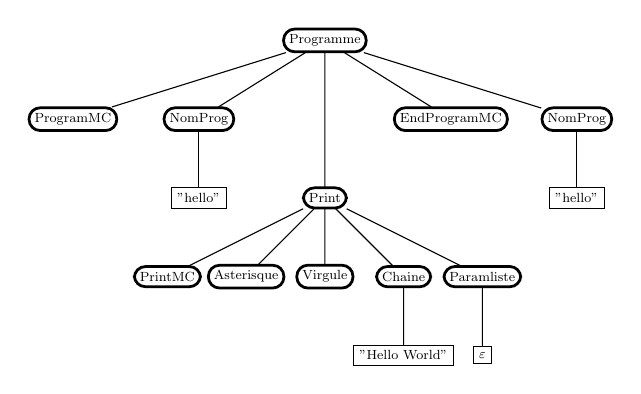
\begin{tikzpicture}[
        baseline=(base), 
        level/.style={sibling distance = 1.6cm/#1, level distance = 1cm},
        every node/.style={scale=0.6, font=\footnotesize}
    ]
    
    \node[ noeud] {Programme}
    child { 
        node[noeud] (base) {ProgramMC}
    }
    child {
        node[noeud] {NomProg}
        child {node[feuille] {"hello"}}
    }
    child [ level distance=2cm]{ 
        node [ noeud] {Print}
        child [sibling distance= 1cm] {
            node [noeud] {PrintMC}
        }
        child [sibling distance= 1cm]{
            node [noeud] {Asterisque}
        }
        child [sibling distance= 1cm]{
            node [noeud] {Virgule}
        }
        child [sibling distance= 1cm]{
            node [noeud] {Chaine}
            child { 
                node [feuille] {"Hello World"}
            }
        }
        child [sibling distance= 1cm] {
            node [noeud] {Paramliste}
            child { 
                node [feuille] {$\varepsilon$}
            }
        }
    }
    child { 
        node[ noeud] {EndProgramMC}
    }
    child {
        node[noeud] {NomProg}
        child {node[feuille] {"hello"}}
    };

\end{tikzpicture}
        }

    \end{center}
\end{frame}



\begin{frame}
    \frametitle{Conversion en arbre de syntaxe abstraite\esp}
    \begin{tikzpicture}
    
    \tikzstyle{lien} = [->, >=latex]
    \tikzstyle{basic_text}=[text width=2cm, text badly centered]
    \tikzstyle{basic_node}=[draw = black,rounded corners=4pt, basic_text]
    \tikzstyle{wrapper}=[basic_node, inner sep=3pt]
    \tikzstyle{hidden}=[draw=black!0,color=black!0]
    \tikzstyle{faded}=[draw=black!20, color=black!20]
    

    \node [basic_node, text width=6cm, align=left] (AS) {
         \scalebox{0.7}{
            \parbox{\textwidth}{
                    
\tikzstyle{feuille}=[ draw, rectangle, inner sep = 0.12cm]
\tikzstyle{noeud}=[ draw, rectangle,rounded corners, minimum width= 0.64cm, line width = 1pt]
\begin{tikzpicture}[
        baseline=(base), 
        level/.style={sibling distance = 1.6cm/#1, level distance = 1cm},
        every node/.style={scale=0.6, font=\footnotesize}
    ]
    
    \node[ noeud] {Programme}
    child { 
        node[noeud] (base) {ProgramMC}
    }
    child {
        node[noeud] {NomProg}
        child {node[feuille] {"hello"}}
    }
    child [ level distance=2cm]{ 
        node [ noeud] {Print}
        child [sibling distance= 1cm] {
            node [noeud] {PrintMC}
        }
        child [sibling distance= 1cm]{
            node [noeud] {Asterisque}
        }
        child [sibling distance= 1cm]{
            node [noeud] {Virgule}
        }
        child [sibling distance= 1cm]{
            node [noeud] {Chaine}
            child { 
                node [feuille] {"Hello World"}
            }
        }
        child [sibling distance= 1cm] {
            node [noeud] {Paramliste}
            child { 
                node [feuille] {$\varepsilon$}
            }
        }
    }
    child { 
        node[ noeud] {EndProgramMC}
    }
    child {
        node[noeud] {NomProg}
        child {node[feuille] {"hello"}}
    };

\end{tikzpicture}
            }
        }
    };

    \node [basic_node, text width=4cm, align=left] (AST) [right=1cm of AS] {
        \scalebox{0.7}{
            \parbox{\textwidth}{
                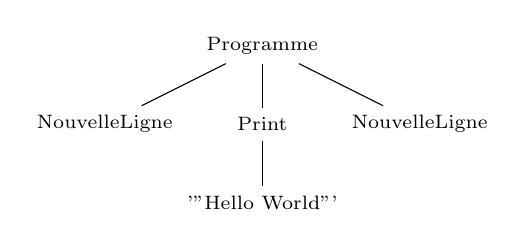
\begin{tikzpicture}
    \node[font=\scriptsize] (0) at (0, 0) {Programme};
    \node[font=\scriptsize] (1) at (-2, -1) {NouvelleLigne};
    \node[font=\scriptsize] (2) at (0, -1) {Print};
    \node[font=\scriptsize] (3) at (0, -2) {'"Hello World"'};
    \node[font=\scriptsize] (4) at (2, -1) {NouvelleLigne};
    
    \draw (0) -- (1);
    \draw (0) -- (2);
    \draw (2) -- (3);
    \draw (0) -- (4);
\end{tikzpicture}
            }
        }
    };
 
    \draw [lien] (AS.north) to[out=45, in=135]  node[midway, above] {\textbf{Conversion en arbre de syntaxe abstraite}}  (AST.north west) ; 

\end{tikzpicture}
\end{frame}


